\chapter{Memory Allocation Strategies}

\section{Introduction}

Memory allocation is the process of assigning portions of memory to programs, processes, threads, kernel subsystems, and data structures. Efficient allocation is critical for performance, scalability, and memory utilization.

Memory allocators aim to balance:

\begin{itemize}
\item Fast allocation
\item Fast deallocation
\item Low fragmentation
\item Good cache locality
\item Scalability on multicore systems
\end{itemize}

\section{Memory Allocation Overview}

Memory allocation occurs at multiple levels:

\begin{enumerate}
\item Physical memory allocation
\item Virtual memory allocation
\item Kernel memory allocation
\item User-space heap allocation
\end{enumerate}

\begin{figure}[H]
\centering
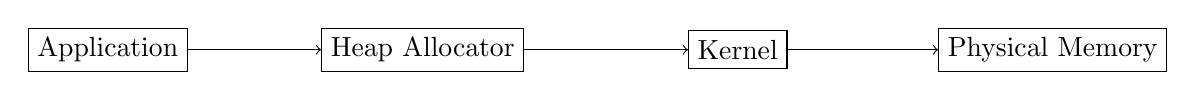
\begin{tikzpicture}
\node[draw] (app) at (0,0) {Application};
\node[draw] (heap) at (4,0) {Heap Allocator};
\node[draw] (kernel) at (8,0) {Kernel};
\node[draw] (ram) at (12,0) {Physical Memory};

\draw[->] (app)--(heap);
\draw[->] (heap)--(kernel);
\draw[->] (kernel)--(ram);
\end{tikzpicture}
\caption{Memory Allocation Layers}
\end{figure}

\section{Fixed Partition Allocation}

Physical memory is divided into fixed-size partitions.

Each process is assigned one partition.

\subsection{Example}

Memory Size:

\[
64\ MB
\]

Partitions:

\[
16\ MB,\ 16\ MB,\ 16\ MB,\ 16\ MB
\]

\begin{figure}[H]
\centering
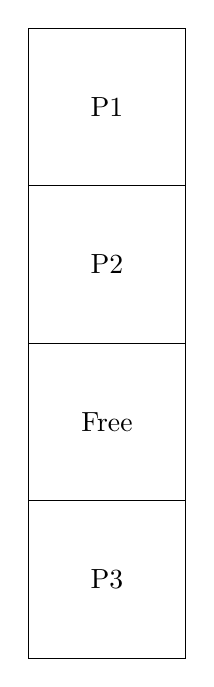
\begin{tikzpicture}
\draw (0,0) rectangle (2,8);

\foreach \y in {2,4,6}
{
\draw (0,\y)--(2,\y);
}

\node at (1,7) {P1};
\node at (1,5) {P2};
\node at (1,3) {Free};
\node at (1,1) {P3};
\end{tikzpicture}
\caption{Fixed Partition Allocation}
\end{figure}

\subsection{Advantages}

\begin{itemize}
\item Simple implementation
\item Fast allocation
\end{itemize}

\subsection{Disadvantages}

\begin{itemize}
\item Internal fragmentation
\item Limited flexibility
\end{itemize}

\section{Dynamic Partition Allocation}

Partitions are created dynamically according to process requirements.

\subsection{Example}

Processes:

\[
10MB,\ 20MB,\ 15MB
\]

Memory allocated exactly as needed.

\begin{figure}[H]
\centering
\begin{tikzpicture}
\draw (0,0) rectangle (2,10);

\draw (0,2)--(2,2);
\draw (0,5)--(2,5);
\draw (0,7)--(2,7);

\node at (1,8.5) {Free};
\node at (1,6) {P3};
\node at (1,3.5) {P2};
\node at (1,1) {P1};
\end{tikzpicture}
\caption{Dynamic Partition Allocation}
\end{figure}

\subsection{Advantages}

\begin{itemize}
\item Better utilization
\item Flexible sizing
\end{itemize}

\subsection{Disadvantages}

\begin{itemize}
\item External fragmentation
\end{itemize}

\section{First Fit}

Allocate the first free block large enough to satisfy the request.

\subsection{Example}

Free blocks:

\[
100,\ 500,\ 200,\ 300,\ 600
\]

Request:

\[
212
\]

Allocated from:

\[
500
\]

Remaining:

\[
288
\]

\subsection{Advantages}

\begin{itemize}
\item Fast
\item Simple
\end{itemize}

\subsection{Disadvantages}

\begin{itemize}
\item Fragmentation near beginning
\end{itemize}

\section{Best Fit}

Allocate the smallest free block that satisfies the request.

\subsection{Example}

Blocks:

\[
100,\ 500,\ 200,\ 300,\ 600
\]

Request:

\[
212
\]

Chosen block:

\[
300
\]

Remaining:

\[
88
\]

\subsection{Advantages}

\begin{itemize}
\item Less wasted space per allocation
\end{itemize}

\subsection{Disadvantages}

\begin{itemize}
\item Slower search
\item Many tiny fragments
\end{itemize}

\section{Worst Fit}

Allocate the largest available block.

\subsection{Example}

Request:

\[
212
\]

Chosen block:

\[
600
\]

Remaining:

\[
388
\]

\subsection{Advantages}

\begin{itemize}
\item Leaves large usable blocks
\end{itemize}

\subsection{Disadvantages}

\begin{itemize}
\item Generally poor utilization
\end{itemize}

\section{Next Fit}

Variation of First Fit.

Search begins from the last allocated location.

\begin{figure}[H]
\centering
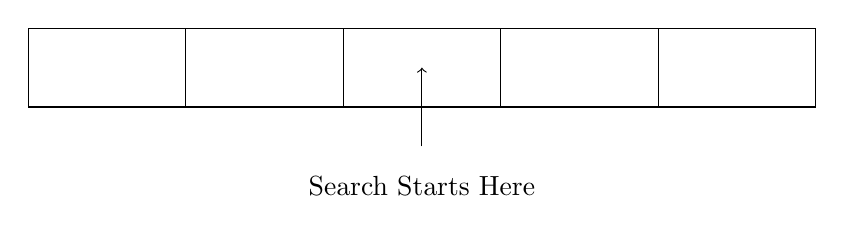
\begin{tikzpicture}
\draw (0,0) rectangle (10,1);

\draw (2,0)--(2,1);
\draw (4,0)--(4,1);
\draw (6,0)--(6,1);
\draw (8,0)--(8,1);

\node at (5,-1) {Search Starts Here};
\draw[->] (5,-0.5)--(5,0.5);
\end{tikzpicture}
\caption{Next Fit Search}
\end{figure}

\subsection{Advantages}

\begin{itemize}
\item Avoids repeated scanning
\end{itemize}

\subsection{Disadvantages}

\begin{itemize}
\item Can increase fragmentation
\end{itemize}

\section{Buddy System}

Memory is managed in power-of-two blocks.

Available sizes:

\[
2^k
\]

Example:

\[
1024KB
\]

Split into:

\[
512 + 512
\]

Then:

\[
256 + 256
\]

Until suitable size found.

\begin{figure}[H]
\centering
\begin{tikzpicture}
\node at (0,0) {1024};

\node at (-2,-2) {512};
\node at (2,-2) {512};

\node at (-3,-4) {256};
\node at (-1,-4) {256};

\draw (0,-0.2)--(-2,-1.8);
\draw (0,-0.2)--(2,-1.8);

\draw (-2,-2.2)--(-3,-3.8);
\draw (-2,-2.2)--(-1,-3.8);
\end{tikzpicture}
\caption{Buddy Allocation Splitting}
\end{figure}

\subsection{Advantages}

\begin{itemize}
\item Fast splitting
\item Fast merging
\end{itemize}

\subsection{Disadvantages}

\begin{itemize}
\item Internal fragmentation
\end{itemize}

\section{Slab Allocation}

Used heavily in kernels.

Stores pre-allocated objects of identical size.

Examples:

\begin{itemize}
\item Process descriptors
\item Inodes
\item File structures
\end{itemize}

\begin{figure}[H]
\centering
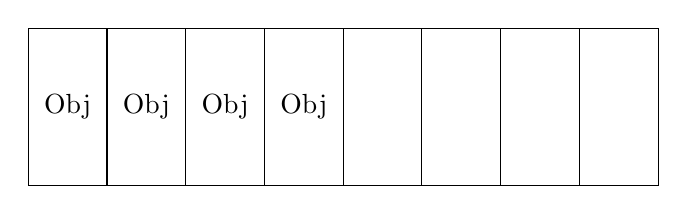
\begin{tikzpicture}
\draw (0,0) rectangle (8,2);

\foreach \x in {1,2,3,4,5,6,7}
{
\draw (\x,0)--(\x,2);
}

\node at (0.5,1) {Obj};
\node at (1.5,1) {Obj};
\node at (2.5,1) {Obj};
\node at (3.5,1) {Obj};
\end{tikzpicture}
\caption{Slab Allocator}
\end{figure}

\subsection{Advantages}

\begin{itemize}
\item Low overhead
\item Excellent cache locality
\item Reduced fragmentation
\end{itemize}

\section{Kernel Memory Allocation}

Kernel allocations differ from user-space allocations.

Requirements:

\begin{itemize}
\item Low latency
\item Predictability
\item Concurrency support
\end{itemize}

Kernel allocators often use:

\begin{itemize}
\item Buddy allocator
\item Slab allocator
\item SLUB
\item SLOB
\end{itemize}

\section{Heap Management}

Heap stores dynamically allocated memory.

Common operations:

\begin{itemize}
\item malloc()
\item calloc()
\item realloc()
\item free()
\end{itemize}

\begin{figure}[H]
\centering
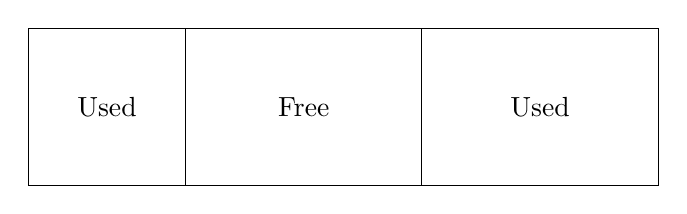
\begin{tikzpicture}
\draw (0,0) rectangle (8,2);

\draw (2,0)--(2,2);
\draw (5,0)--(5,2);

\node at (1,1) {Used};
\node at (3.5,1) {Free};
\node at (6.5,1) {Used};
\end{tikzpicture}
\caption{Heap Layout}
\end{figure}

\section{Free Lists}

Free memory blocks are maintained in linked lists.

\subsection{Example}

\[
100 \rightarrow 200 \rightarrow 500 \rightarrow 300
\]

Allocation traverses the list to find a suitable block.

\subsection{Advantages}

\begin{itemize}
\item Simple
\item Flexible
\end{itemize}

\subsection{Disadvantages}

\begin{itemize}
\item Search overhead
\end{itemize}

\section{Fragmentation Analysis}

\subsection{Internal Fragmentation}

Allocated block larger than requested.

Example:

\[
Request=10KB
\]

\[
Allocated=16KB
\]

Waste:

\[
6KB
\]

\subsection{External Fragmentation}

Enough total memory exists but is scattered.

\begin{figure}[H]
\centering
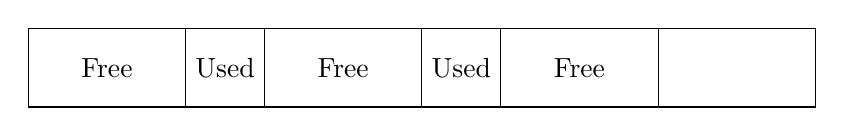
\begin{tikzpicture}
\draw (0,0) rectangle (10,1);

\draw (2,0)--(2,1);
\draw (3,0)--(3,1);
\draw (5,0)--(5,1);
\draw (6,0)--(6,1);
\draw (8,0)--(8,1);

\node at (1,0.5) {Free};
\node at (2.5,0.5) {Used};
\node at (4,0.5) {Free};
\node at (5.5,0.5) {Used};
\node at (7,0.5) {Free};
\end{tikzpicture}
\caption{External Fragmentation}
\end{figure}

\section{Memory Pools}

Preallocated memory regions for fixed-size allocations.

Advantages:

\begin{itemize}
\item Constant-time allocation
\item Predictable performance
\item Reduced fragmentation
\end{itemize}

Used in:

\begin{itemize}
\item Game engines
\item Networking systems
\item Embedded systems
\end{itemize}

\section{Allocators in Modern Systems}

Modern allocators emphasize:

\begin{itemize}
\item Thread scalability
\item NUMA awareness
\item Cache locality
\item Low contention
\end{itemize}

Features:

\begin{itemize}
\item Per-thread caches
\item Lock-free structures
\item Object reuse
\end{itemize}

\section{Linux Memory Allocation}

Linux uses multiple allocators.

Physical memory:

\begin{itemize}
\item Buddy allocator
\end{itemize}

Kernel objects:

\begin{itemize}
\item SLAB
\item SLUB
\item SLOB
\end{itemize}

User-space:

\begin{itemize}
\item glibc malloc
\item jemalloc
\item tcmalloc
\end{itemize}

\section{malloc Internals Overview}

Typical malloc implementation:

\begin{enumerate}
\item Request arrives
\item Search free list/bin
\item Split large block if necessary
\item Return pointer
\item Merge adjacent blocks on free
\end{enumerate}

\subsection{Common Data Structures}

\begin{itemize}
\item Free lists
\item Bins
\item Arenas
\item Metadata headers
\end{itemize}

\section{jemalloc and tcmalloc Overview}

\subsection{jemalloc}

Developed for scalability.

Features:

\begin{itemize}
\item Multiple arenas
\item Reduced lock contention
\item Good fragmentation behavior
\end{itemize}

Used by:

\begin{itemize}
\item FreeBSD
\item Firefox
\item Various databases
\end{itemize}

\subsection{tcmalloc}

Developed by Google.

Features:

\begin{itemize}
\item Thread-local caches
\item Fast allocation
\item Efficient multicore scaling
\end{itemize}

Used by:

\begin{itemize}
\item Large-scale backend systems
\item Performance-sensitive services
\end{itemize}

\section{Detailed Comparison of Allocation Methods}

\begin{center}
\begin{tabular}{p{2.8cm}p{2.8cm}p{2.8cm}p{2.8cm}p{2.8cm}}
\toprule
Method & Speed & Fragmentation & Complexity & Typical Usage \\
\midrule
Fixed Partition & High & Internal & Low & Legacy Systems \\
Dynamic Partition & Medium & External & Medium & General Allocation \\
First Fit & High & Medium & Low & OS Allocation \\
Best Fit & Low & High Tiny Fragments & Medium & Research \\
Worst Fit & Medium & High & Medium & Educational \\
Next Fit & Medium & Medium & Low & Variants \\
Buddy & High & Internal & Medium & Kernel Memory \\
Slab & Very High & Very Low & Medium & Kernel Objects \\
Memory Pool & Very High & Low & Medium & Real-Time Systems \\
jemalloc & Very High & Low & High & Servers \\
tcmalloc & Very High & Low & High & Large Services \\
\bottomrule
\end{tabular}
\end{center}

\section{Performance Analysis}

\begin{center}
\begin{tabular}{lll}
\toprule
Allocator & Allocation Speed & Scalability \\
\midrule
First Fit & Good & Moderate \\
Best Fit & Poor & Moderate \\
Buddy & Good & Good \\
Slab & Excellent & Excellent \\
jemalloc & Excellent & Excellent \\
tcmalloc & Excellent & Excellent \\
\bottomrule
\end{tabular}
\end{center}

\section{Interview Discussions}

\subsection{Why is Buddy Allocation Popular in Kernels?}

\begin{itemize}
\item Fast splitting
\item Fast merging
\item Efficient physical page management
\end{itemize}

\subsection{Why is Slab Allocation Used?}

\begin{itemize}
\item Frequent object reuse
\item Better cache locality
\item Lower fragmentation
\end{itemize}

\subsection{Why Do Modern Servers Use jemalloc or tcmalloc?}

\begin{itemize}
\item Better multicore scalability
\item Reduced contention
\item Improved performance
\end{itemize}

\section{Key Takeaways}

\begin{keytakeaways}
Memory allocation strategies differ in speed, fragmentation characteristics, and scalability. First Fit is simple and fast, Best Fit minimizes immediate waste but may increase fragmentation, and Worst Fit is rarely used in practice. Buddy allocation efficiently manages physical memory, while Slab allocation is ideal for frequently used kernel objects. Modern allocators such as jemalloc and tcmalloc are optimized for multicore scalability, low contention, and improved cache locality.
\end{keytakeaways}

\section{Interview Questions with Answers}

\begin{enumerate}
\item What is memory allocation?\\
Assigning memory blocks to processes or data structures.

\item What is fixed partition allocation?\\
Memory divided into predefined partitions.

\item Main drawback of fixed partitions?\\
Internal fragmentation.

\item What is dynamic partition allocation?\\
Partitions created based on process size.

\item What is First Fit?\\
Allocate first sufficiently large block.

\item What is Best Fit?\\
Allocate smallest suitable block.

\item What is Worst Fit?\\
Allocate largest available block.

\item What is Next Fit?\\
First Fit starting from last allocation point.

\item What is the Buddy System?\\
Power-of-two memory allocator.

\item Why is Buddy Allocation efficient?\\
Fast splitting and merging.

\item What is Slab Allocation?\\
Allocator for fixed-size kernel objects.

\item Why use Slab Allocation?\\
Reduced fragmentation and better locality.

\item What is heap memory?\\
Dynamic memory allocation area.

\item What is a free list?\\
List of available memory blocks.

\item What is internal fragmentation?\\
Unused space inside allocated blocks.

\item What is external fragmentation?\\
Free memory scattered into small pieces.

\item What is a memory pool?\\
Preallocated memory region.

\item What allocator manages physical memory in Linux?\\
Buddy allocator.

\item What is jemalloc?\\
Scalable high-performance memory allocator.

\item What is tcmalloc?\\
Google's thread-caching allocator.
\end{enumerate}

\section{MCQs with Answers}

\begin{enumerate}
\item Fixed partition allocation suffers from:
\begin{enumerate}[label=(\alph*)]
\item External Fragmentation
\item Internal Fragmentation
\item Thrashing
\item Deadlock
\end{enumerate}
Answer: (b)

\item Dynamic partition allocation suffers from:
\begin{enumerate}[label=(\alph*)]
\item External Fragmentation
\item Internal Fragmentation
\item Starvation
\item Deadlock
\end{enumerate}
Answer: (a)

\item First Fit allocates:
\begin{enumerate}[label=(\alph*)]
\item Largest Block
\item Smallest Block
\item First Suitable Block
\item Last Suitable Block
\end{enumerate}
Answer: (c)

\item Best Fit chooses:
\begin{enumerate}[label=(\alph*)]
\item Largest Block
\item Smallest Suitable Block
\item First Block
\item Random Block
\end{enumerate}
Answer: (b)

\item Worst Fit chooses:
\begin{enumerate}[label=(\alph*)]
\item Largest Block
\item Smallest Block
\item First Block
\item Random Block
\end{enumerate}
Answer: (a)

\item Next Fit starts searching from:
\begin{enumerate}[label=(\alph*)]
\item Beginning
\item End
\item Previous Allocation Point
\item Random Position
\end{enumerate}
Answer: (c)

\item Buddy allocation uses:
\begin{enumerate}[label=(\alph*)]
\item Prime Numbers
\item Fibonacci Sizes
\item Powers of Two
\item Linked Pages
\end{enumerate}
Answer: (c)

\item Slab allocation is primarily used for:
\begin{enumerate}[label=(\alph*)]
\item Kernel Objects
\item Scheduling
\item DMA
\item Networking Only
\end{enumerate}
Answer: (a)

\item Heap memory supports:
\begin{enumerate}[label=(\alph*)]
\item Dynamic Allocation
\item Interrupts
\item Scheduling
\item Context Switching
\end{enumerate}
Answer: (a)

\item malloc allocates memory from:
\begin{enumerate}[label=(\alph*)]
\item Heap
\item Stack
\item Registers
\item Cache
\end{enumerate}
Answer: (a)

\item Internal fragmentation means:
\begin{enumerate}[label=(\alph*)]
\item Wasted Space Within Allocated Block
\item Scattered Free Space
\item Paging Activity
\item Deadlock
\end{enumerate}
Answer: (a)

\item External fragmentation means:
\begin{enumerate}[label=(\alph*)]
\item Wasted Internal Space
\item Scattered Free Space
\item Context Switch
\item DMA Transfer
\end{enumerate}
Answer: (b)

\item Linux physical memory allocator:
\begin{enumerate}[label=(\alph*)]
\item Buddy
\item Slab
\item malloc
\item JVM
\end{enumerate}
Answer: (a)

\item SLUB is a:
\begin{enumerate}[label=(\alph*)]
\item Kernel Allocator
\item Scheduler
\item Filesystem
\item Protocol
\end{enumerate}
Answer: (a)

\item Memory pools provide:
\begin{enumerate}[label=(\alph*)]
\item Predictable Allocation
\item Slower Allocation
\item More Paging
\item More Fragmentation
\end{enumerate}
Answer: (a)

\item jemalloc focuses on:
\begin{enumerate}[label=(\alph*)]
\item Scalability
\item Compilation
\item Scheduling
\item Paging
\end{enumerate}
Answer: (a)

\item tcmalloc was developed by:
\begin{enumerate}[label=(\alph*)]
\item Microsoft
\item IBM
\item Google
\item Oracle
\end{enumerate}
Answer: (c)

\item Free lists store:
\begin{enumerate}[label=(\alph*)]
\item Available Blocks
\item Processes
\item Threads
\item Files
\end{enumerate}
Answer: (a)

\item Slab allocation improves:
\begin{enumerate}[label=(\alph*)]
\item Cache Locality
\item Deadlocks
\item Scheduling
\item Paging
\end{enumerate}
Answer: (a)

\item Modern allocators emphasize:
\begin{enumerate}[label=(\alph*)]
\item Scalability
\item Locality
\item Low Contention
\item All of the Above
\end{enumerate}
Answer: (d)
\end{enumerate}

\section{Revision Notes}

\begin{revisionnotes}
\item Fixed partitions cause internal fragmentation.
\item Dynamic partitions may cause external fragmentation.
\item First Fit is fast and simple.
\item Best Fit minimizes immediate waste.
\item Worst Fit uses the largest block.
\item Next Fit continues searching from the last position.
\item Buddy allocation uses powers of two.
\item Slab allocation is optimized for kernel objects.
\item Heap memory supports dynamic allocation.
\item Free lists track available memory blocks.
\item Internal fragmentation wastes space inside allocations.
\item External fragmentation scatters free memory.
\item Memory pools provide predictable allocation.
\item Linux uses Buddy and Slab-family allocators.
\item jemalloc and tcmalloc target multicore scalability.
\end{revisionnotes}

\section{Cheat Sheet}

\begin{longtable}{|p{5cm}|p{8cm}|}
\hline
Concept & Summary \\
\hline
Fixed Partition & Fixed-size memory regions \\
\hline
Dynamic Partition & Variable-size regions \\
\hline
First Fit & First suitable block \\
\hline
Best Fit & Smallest suitable block \\
\hline
Worst Fit & Largest available block \\
\hline
Next Fit & Continue from previous position \\
\hline
Buddy System & Power-of-two allocation \\
\hline
Slab Allocation & Fixed-size kernel objects \\
\hline
Heap & Dynamic allocation region \\
\hline
Free List & Available block tracking \\
\hline
Internal Fragmentation & Waste inside allocation \\
\hline
External Fragmentation & Scattered free memory \\
\hline
Memory Pool & Preallocated region \\
\hline
Linux Physical Allocator & Buddy Allocator \\
\hline
Kernel Object Allocator & Slab / SLUB \\
\hline
malloc & User-space heap allocator \\
\hline
jemalloc & Scalable allocator \\
\hline
tcmalloc & Thread-caching allocator \\
\hline
Best Kernel Allocator & Slab-family allocators \\
\hline
Most Asked Interview Topic & Buddy vs Slab Allocation \\
\hline
\end{longtable}